In this session, we will describe VD's data and settings, show the performance of VD on primary tasks, and introduce several derived applications empowered by the multi-flow multimodal property of VD.

\begin{figure*}[t]
    \centering
    \begin{subfigure}[b]{0.92\textwidth}
        \centering
        \includegraphics[width=\textwidth]{figure/qcompare1.pdf}
        \caption{Text-to-Image performance.}
        \vspace{0.2cm}
        \label{fig:qcompare_t2i}
    \end{subfigure}
    
    \begin{subfigure}[b]{0.92\textwidth}
        \centering
        \includegraphics[width=\textwidth]{figure/qcompare2.pdf}
        \caption{Image-Variation performance.}
        \vspace{0.2cm}
        \label{fig:qcompare_i2i}
    \end{subfigure}
    \begin{subfigure}[b]{0.92\textwidth}
        \centering
        \includegraphics[width=\textwidth]{figure/qcompare3-small.pdf}
        \caption{Image-to-Text performance.}
        \vspace{0.1cm}
        \label{fig:qcompare_i2t}
    \end{subfigure}
    
    \caption{
        These figures show the qualitative comparison between our VD models and prior works, from which we conclude that VD performs well on all three tasks. In text-to-image and image-variation, VD captures semantics from the input context more accurately. In image-to-text, VD generates more creative sentences and has a better chance to describe images with more details.
    }
    \label{fig:qcompare}
\end{figure*}


\subsection{Dataset}

We used Laion2B-en~\cite{laion} and COYO-700M~\cite{coyo} as VD's train data. Both Laion2B and COYO are collections of image-text pairs in English, in which images are collected from websites, and the corresponding captions are excerpted from HTML pages. We further filtered all data with the following criteria: a) image-text CLIP similarity scores above 0.3; b) safety scores (\ie NSWF) below 0.3; c) the probability containing watermark below 0.3; d) image aspect ratios within 0.6 to 1.6667; e) image area above $256^2 \times 0.75$. These filtered samples served as the train data for all our VD experiments. Besides, we noticed that the web crawling captions tend to be noisy, so we cleaned them with a customized algorithm described in Appendix~\ref{sec:supp_prompt_clearning}. 

\subsection{Training}

We trained VD progressively with three settings: single-flow, dual-flow, and four-flow, among which the single-flow is an image-variation model; the dual-flow is a text-to-image and image-variation model; and the four-flow is the main VD model with four tasks we majorly described in this work. During training, we kept diffusion settings close to DDPM~\cite{ddpm} and SD~\cite{ldm}, \ie, 1000 diffusion steps and linearly increasing $\beta$ from $8.5e-5$ to $1.2e-2$ according to steps. The learning rates were set to $1.e-4$ for single-flow and dual-flow, and were set to $5.e-5$ for four-flow. The single-flow model used SD checkpoint v1.4~\cite{ldm} as its initial weights, and others continued finetuning the latest checkpoint from the previous models. During training, we set different gradient scales for different layers to best cooperate with the initial weights. One can find these details in Table~\ref{table:gmsetting}. The effective batch size was 2048 for single-flow, 1024 for dual-flow, and 512 for four-flow. The logic behind the learning rates, batch sizes, and gradient scales is to roughly balance each gradient step while training. All models were trained with 30 million samples on resolution 256, followed by 6.4 million samples on resolution 512. Compared with SDv1.4, which was trained on 500 plus 230 million samples on resolutions 256 and 512, VD's training cost is more affordable, benefiting researchers in the long run.

\begin{table}[h!]
\centering
\resizebox{0.9\columnwidth}{!}{
    \begin{tabular}{
            C{1.8cm}
            C{1.2cm}
            C{1.2cm}
            C{1cm}
            C{1cm}
            C{1cm}}
        \toprule
            & Data(I) & Data(T)
            & Ctx(I) & Ctx(T)
            & Global
            \\
        \midrule
        VD (1-flow)
            & 0.1
            & --
            & 1.0
            & --
            & 0.1
            \\
        VD (2-flow)
            & 0.1
            & --
            & 1.0
            & 1.0
            & 0.1
            \\
        VD (4-flow)
            & 0.2
            & 1.0
            & 1.0
            & 1.0
            & 0.1
            \\
        \bottomrule
    \end{tabular}
}
\vspace{0.3cm}
\caption{
    This table shows the gradient scales used by different layers when training various settings of VD. Data(I) means the image data layer, so on and so forth.
}
\label{table:gmsetting}
\end{table}

\subsection{Performance}

To the best of our knowledge, VD is the first image-text multi-flow multimodal model that can be evaluated across different tasks. Thus, we chose single-task-focused prior works as our baselines when comparing the performance. Explicitly speaking: we chose SDv1.4~\cite{ldm} as our text-to-image baseline; SD-variation~\cite{sd-justin} (\ie a finetuned SD for image-variation) as our image-variation baseline; and BLIP~\cite{blip} as our image-to-text baseline. We conducted both qualitative and quantitative comparisons between baselines and various versions of VD, \ie, dual-flow and four-flow for text-to-image, and all three models for image-variation. Although DALLE2~\cite{dalle2} and Imagen~\cite{imagen} also achieved SOTA on text-to-image, they were not compared because of no publicly available code and model. For image-to-text (\ie image captioning), we only compare BLIP~\cite{blip} with our four-flow VD since other settings do not support this task.

Figure~\ref{fig:qcompare} compares VD's qualitative performance with its baseline, in which images in each row are created with the same random seeds for better quality checks. We also compute text-to-image and image-variation FID scores by comparing 30000 randomly generated samples with the validation set of COCO-caption~\cite{coco}. In Figure~\ref{fig:quant_result}, we list VD's performance along with other related works. We also plot the changes in VD's FID according to the unconditional guidance scale (\ie the classifier-free guidance scale). Lastly, we carried out user studies on 2000 samples from COCO-Caption~\cite{coco} split by four moderators, in which moderators were asked to vote for better quality or ``equally good" (see Figure~\ref{fig:user_study}).

\begin{figure}[t]
\centering
\begin{subfigure}[b]{0.475\columnwidth}
    \resizebox{\columnwidth}{!}{
    \begin{tabular}{
            C{4cm}
            C{2cm}}
        \toprule
            Method & FID $\downarrow$
            \\
        \midrule
        \midrule
            \multicolumn{2}{c}{(A) Text-to-Image Synthesis}
            \\
        \midrule
            CogView~\cite{cogview} & 27.10 \\
            LAFITE~\cite{lafite}  & 26.94 \\
            GLIDE~\cite{glide}   & 12.24 \\
            Make-a-Scene~\cite{mask-a-scene} & 11.84 \\
            LDM~\cite{ldm} & 12.63 \\
            SD (baseline) & 11.21 \scriptsize{$\pm$0.03} \\
            \textbf{VD (four-flow)} & \textbf{11.10 \scriptsize{$\pm$0.09}} \\
        \midrule
        \midrule
            \multicolumn{2}{c}{(B) Image-Variation Synthesis}
            \\
        \midrule
            SD (baseline) & 18.81 \scriptsize{$\pm$0.06} \\
            \textbf{VD (four-flow)} & \textbf{4.57 \scriptsize{$\pm$0.02}} \\
        \bottomrule
    \end{tabular}
}

    % \subcaption{
    %     \scriptsize VD text-to-image and image-variation FID compared with baseline and prior approaches.
    % }
\end{subfigure}
\hfill
\begin{subfigure}[b]{0.475\columnwidth}
    \resizebox{\columnwidth}{!}{
    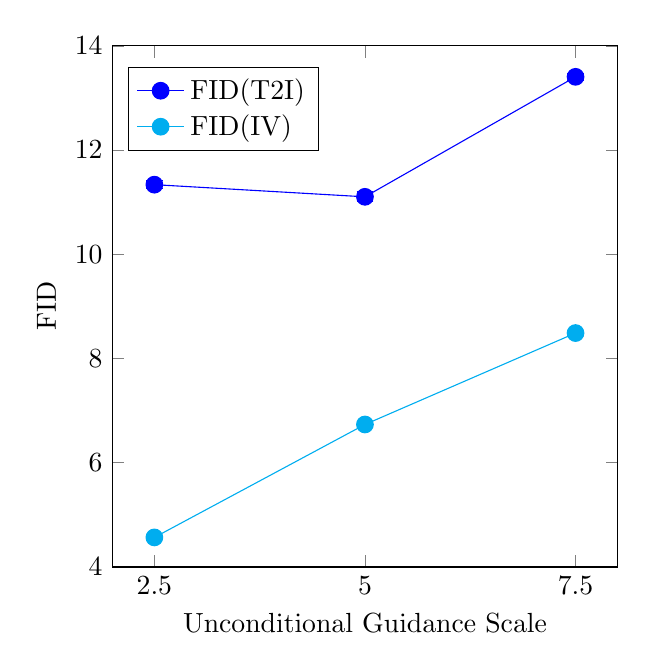
\begin{tikzpicture}
    \begin{axis}[
        xlabel=Unconditional Guidance Scale,
        ylabel=FID,
        xmin=2,
        xmax=8,
        ymin=4,
        ymax=14,
        xtick={2.5,5.0,7.5},
        width=8cm,height=8.2cm,
        legend style={at={(0.22,0.96)},anchor=north,legend cell align=left},
    ]
    \addplot+[
        blue,
        mark=*, mark size=3pt, mark options={fill=blue},
        error bars/.cd,y dir=both,y explicit,
    ] coordinates {
        (2.5, 11.3355988257) +- (0, 0.0796762530121)
        (5.0, 11.1023553055) +- (0, 0.0916626027159)
        (7.5, 13.405008415)  +- (0, 0.0681356441779)
    };\label{t2i-fid}\addlegendentry{FID(T2I)}
    \addplot+[
        cyan,
        mark=*, mark size=3pt, mark options={fill=cyan},
        error bars/.cd,y dir=both,y explicit,
    ] coordinates {
        (2.5, 4.56646982092) +- (0, 0.0211169100996)
        (5.0, 6.7336671616) +- (0, 0.0299270554132)
        (7.5, 8.48817909203)  +- (0, 0.0205315863737)
    };\label{iv-fid}\addlegendentry{FID(IV)}
    \end{axis}
    \end{tikzpicture}
}
    \vspace{-0.9cm}
    % \subcaption{
    %     \scriptsize VD text-to-image and image-variation FID under different classifier-free guidance scales.
    % }
\end{subfigure}
\caption{FID scores of VD comparing with baseline and prior approaches, and under various unconditional (classifier-free) guidance scales.}
\label{fig:quant_result}
\end{figure}

\begin{figure}[t]
\centering
\begin{subfigure}[b]{0.475\columnwidth}
    \resizebox{\columnwidth}{!}{
        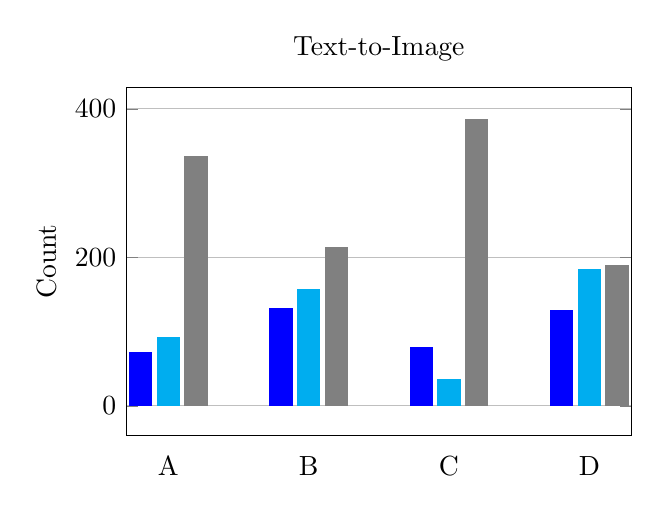
\begin{tikzpicture}
            \begin{axis}[
                major x tick style = transparent,
                ybar,
                bar width=8pt,
                ymajorgrids = true,
                width=8cm,height=6cm,
                title=Text-to-Image,
                % xlabel = Moderators,
                ylabel = Count,
                symbolic x coords={A,B,C,D},
                xtick = data,
                scaled y ticks = false,
                ymin = -40,
            ]
                \addplot[style={blue,fill=blue,mark=none}]
                    coordinates {(A,72) (B,131) (C,79) (D,128)};
        
                \addplot[style={cyan,fill=cyan,mark=none}]
                    coordinates {(A,92) (B,156) (C,35) (D,183)};
        
                \addplot[style={gray,fill=gray,mark=none}]
                    coordinates {(A,336) (B,213) (C,386) (D,189)};
                \end{axis}
        \end{tikzpicture}
    }
\end{subfigure}
\hfill
\begin{subfigure}[b]{0.475\columnwidth}
    \resizebox{\columnwidth}{!}{
        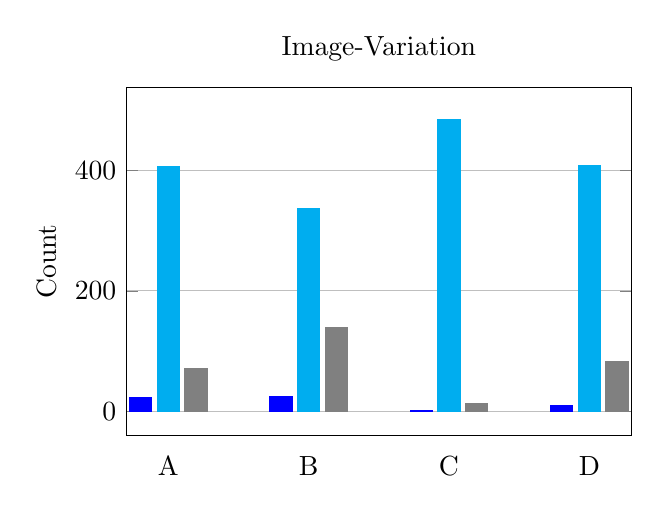
\begin{tikzpicture}
            \begin{axis}[
                major x tick style = transparent,
                ybar,
                bar width=8pt,
                ymajorgrids = true,
                width=8cm,height=6cm,
                title=Image-Variation,
                % xlabel = Moderators,
                ylabel = Count,
                symbolic x coords={A,B,C,D},
                xtick = data,
                scaled y ticks = false,
                ymin = -40,
            ]
                \addplot[style={blue,fill=blue,mark=none}]
                    coordinates {(A,23) (B,25) (C,2) (D,10)};
        
                \addplot[style={cyan,fill=cyan,mark=none}]
                    coordinates {(A,406) (B,336) (C,485) (D,408)};
        
                \addplot[style={gray,fill=gray,mark=none}]
                    coordinates {(A,71) (B,139) (C,13) (D,82)};
                \end{axis}
        \end{tikzpicture}
    }
\end{subfigure}
\caption{User studies on text-to-image and image-variation in which we count the votes from 4 individual moderators on SD (\textcolor{blue}{blue}), VD (\textcolor{cyan}{cyan}), or equally good (\textcolor{gray}{gray}).}
\vspace{-0.2cm}
\label{fig:user_study}
\end{figure}

Through all results, we not only demonstrated that VD outperforms its baseline on these primary tasks, but reveals the effectiveness of our multi-flow multimodal diffusion framework in which context and data with distinct modalities can be analyzed and generated in one unified model.

\subsection{Disentanglement of style and semantic}

One exciting discovery of our VD is that it can enhance or reduce image styles from semantics without further supervision. Such a phenomenon inspires us to explore a novel area where disentanglement between styles and semantics can happen on images with arbitrary contents in arbitrary styles. Recall that prior works such as~\cite{gan_dissect, ganspace} explored similar properties in GAN latent spaces, but their domain of study was restricted to well-aligned data such as faces or churches. To our best knowledge, we are the first group exploring: a) unsupervised semantic and style disentanglement on natural images without domain specifications; b) semantic and style disentanglement on diffusion models' latent space.

Figure~\ref{fig:disentanglement} shows the disentanglement results of VD. In practice, we notice that both two-flow and four-flow models serve similar performance, while single-flow has slightly lower performance. This may be due to the caption-agnostic and insufficient training that reduced the model's capacity. More details and analysis can be found in Appendix~\ref{sec:supp_disentanglement}.

\begin{figure}[t]
    \centering
    \includegraphics[width=0.48\textwidth]{main_figure/disentanglement.pdf}
    \vspace{-0.4cm}
    \caption{Our VD can disentangle image semantics from styles and vice versa. In this figure, we first generate variations of the input images and then manipulate them focused on either semantics (to the left) or styles (to the right).}
    \label{fig:disentanglement}
\end{figure}

\begin{figure}[t]
    \centering
    \includegraphics[width=0.48\textwidth]{figure/dual_guidance.pdf}
    \vspace{-0.2cm}
    \caption{This figure shows image samples created with the dual-guidance of text prompts and reference images (left). Image samples without borders are baseline results generated by ensembling SDv1.4~\cite{ldm} with SD-variation~\cite{sd-justin}. Image samples with green borders are VD's outputs (ours) with attention-level mixing. To fairly compare the performance, samples in one columns have the exact same random seed and thus the same diffusion noises.}
    \label{fig:dual_guidance}
\end{figure}

\subsection{Dual- and multi-context blender}

Since VD is a unified model for multiple tasks, generation from multi-context becomes a natural extension for VD. Recall that a baseline multi-context generation can be achieved by mixing up diffusion steps from distinct models~\cite{dm_morecontrol}. However, in practice, we notice such a baseline cannot reach satisfactory results despite doubling the model usage. Figure~\ref{fig:dual_guidance} compares the dual-context results using one text and one image, in which we use the mixing of SDv1.4~\cite{ldm} (text-to-image) and SD-variation~\cite{sd-justin} (image-variation) as our baseline (labeled as SD). One may easily notice that VD generates more natural-looking results with fewer distortions. We believe that the good performance of VD is largely attributed to its multi-flow structure, through which intermediate features generated from different contexts can be merged on a much deeper level (\ie layer-level or attention-level), instead of merged on the shallow model-level between diffusion steps. More details regarding mixing levels can be found in Appendix~\ref{sec:supp_dcg}.

We further expand this task to a more generalized form with multi-context, resulting in the multi-context blender application. The multi-context blender for VD supports an optional text context, several image contexts, and optional image masks in order to guide the generation process with more detail controls. Figure~\ref{fig:multi_context} shows the performance of our multi-context blender. Notice that there are other recent works such as~\cite{p2p, insp2p, controlnet, attend_and_excite, dreambooth, custom_diffusion, imagic} focused on the broader image editing topic. We encourage readers to check our Appendix~\ref{sec:supp_dcg} and~\ref{sec:supp_mcg} for more details and comparisons. 

\begin{figure}[t]
    \centering
    \includegraphics[width=0.46\textwidth]{main_figure/multi_context.pdf}
    \caption{This figure shows images created with VD's multi-context blender in which multiple images with optional text and masks are applied as contexts. One can notice that VD can smoothly transfer and reconstruct semantic from contexts to outputs.}
    \label{fig:multi_context}
\end{figure}
